\documentclass{standalone}
\usepackage{tikz}
\usepackage{color}
\usepackage{bm}
\usepackage{amssymb}
\usepackage{tkz-euclide}
\usetikzlibrary{arrows.meta}
\usetikzlibrary{positioning}
\usetikzlibrary{calc}
\usetikzlibrary{circuits.ee.IEC}

\tikzset{
  row/.style = {rectangle, rounded corners, draw=black, minimum width =40, minimum height =13},
  col/.style = {rectangle, rounded corners, draw=black, minimum width =11, minimum height =36},
  box/.style = {rectangle, rounded corners, draw=black, minimum width =45, minimum height =45},
  encoder/.style = {rectangle, rounded corners, draw=black, fill=blue!5, minimum width=20, minimum height=2cm},
  interactor/.style = {rectangle, rounded corners, draw=black, fill=blue!5, minimum width=15, minimum height=6cm},
  operation/.style= {rectangle, rounded corners, draw=black, dashed, fill=yellow!10, minimum width =16, minimum height =0.5cm},
  circ1/.style = {circle, draw=black, fill=red!30, thin, radius=1},
  circ2/.style = {circle, draw=black, fill=blue!30, thin, radius=1},
  circ3/.style = {circle, draw=black, fill=red!50, thin, radius=1},
  circ4/.style = {circle, draw=black, fill=blue!50, thin, radius=1},
  circ7/.style = {circle, draw=black, fill=gray!40, thin, radius=1},
  circ8/.style = {circle, draw=black, fill=gray!60, thin, radius=1},
  circ9/.style = {circle, draw=black, fill=black!60, thin, radius=1},
  circ10/.style = {circle, draw=black, fill=gray!80, thin, radius=1},
  cell/.style={rectangle,draw=black,thin, minimum size=0.4cm},
  cell2/.style={rectangle,draw=black,thin, minimum size=0.45cm},
  activated/.style={circle, minimum size=0.5cm, draw=red, thick},
  regular/.style={circle, minimum size=0.5cm, draw=black, thick},
  matmul/.style={bulb, scale=1.3, thick},
  line/.style={->,thick},
  dashedBox/.style={rectangle,thick,rounded corners=5pt,dashed,draw=black}
}

\begin{document}
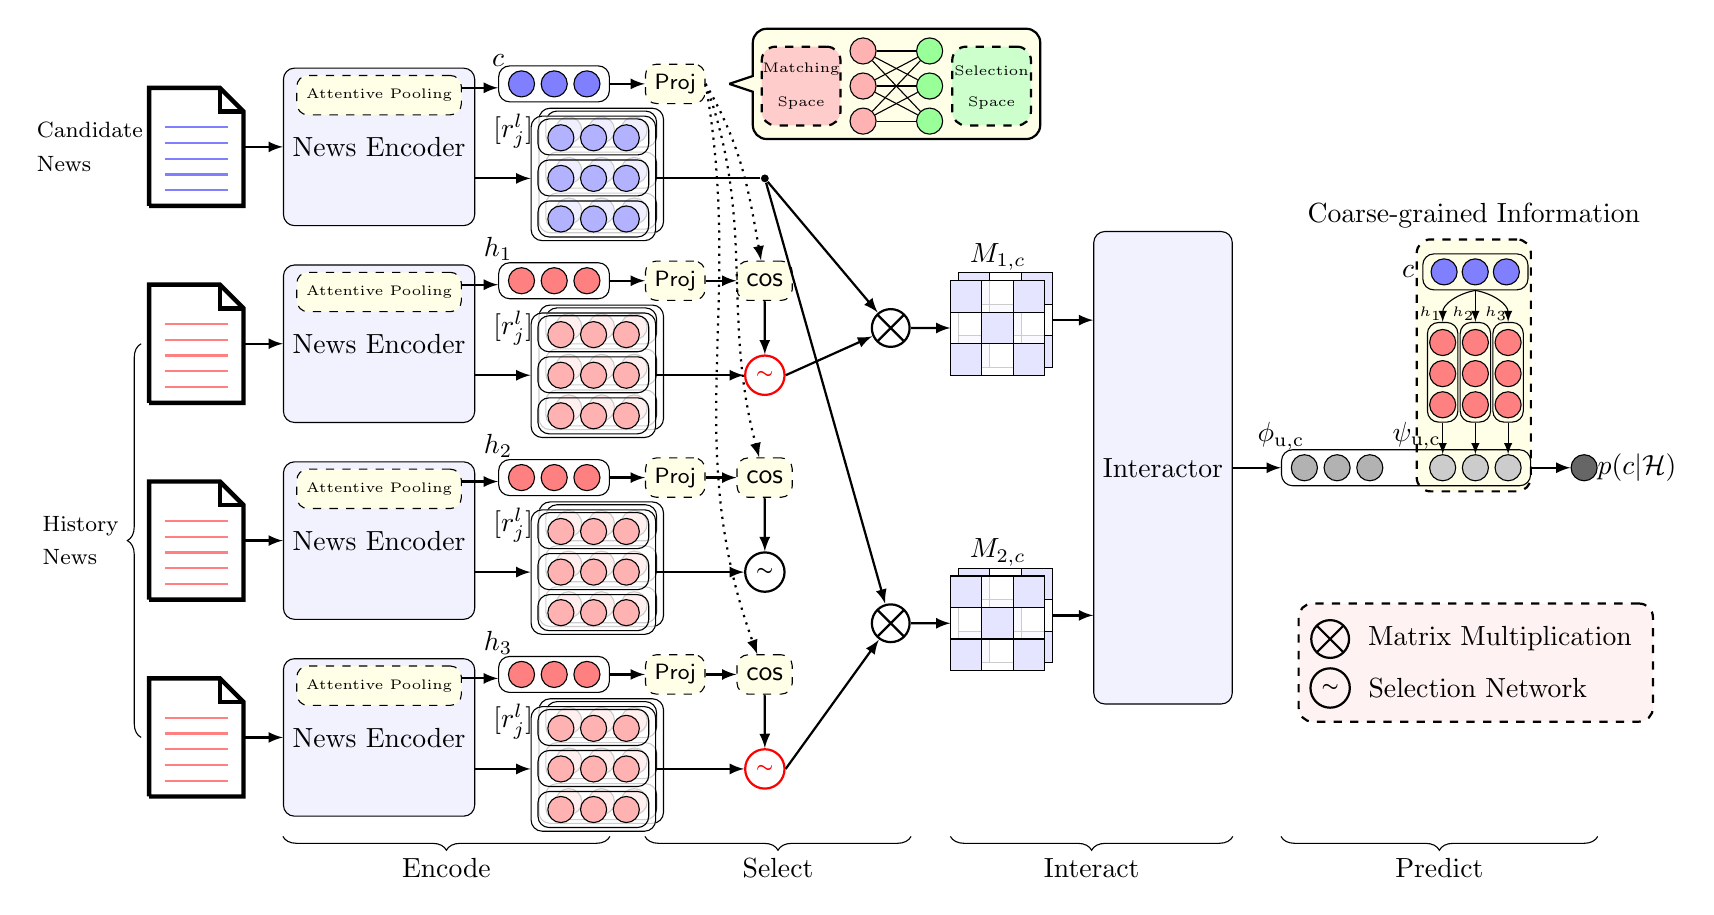
\begin{tikzpicture}[circuit ee IEC,>=latex]
    % \tkzInit[xmax=20,ymax=20,xmin=-3,ymin=-3]
    % \tkzGrid
    % \tkzAxeXY

    \coordinate(disBetweenNews) at (0,1);
    \coordinate(shiftEncoder2Embedding) at (1.6,-0.3);
    \coordinate(shiftEncoder2Repr) at (1,0.8);
    \coordinate(shiftRepr2Trans) at (0.83,0);
    \coordinate(shiftTrans2Dp) at (0.75,0);
    \coordinate(shiftEmbedding2Select) at (1.38,0);
    \coordinate(xshiftSelect2Matmul) at (1.6,0);
    \coordinate(shiftMm2Matrix) at (0.8,-0.3);
    \coordinate(shiftMatrix2Interactor) at (1.4,0);
    \coordinate(shiftInteractor2Vec) at (2.2,0);
    \coordinate(shiftGate2Score) at (0.5,0);


    % news
    \begin{scope}[local bounding box=his3News]
        \draw[ultra thick] (0,0) -- ++(1.2,0) -- ++(0,1.2)-- ++(-0.3,0.3) -- ++(-0.9,0) -- ++(0,-1.5);
        \draw[ultra thick] (0.9,1.5) -- ++(0,-0.3) -- ++(0.3,0);
        \draw[thick,draw=red!50] (0.2,0.2) -- (1,0.2);
        \draw[thick,draw=red!50] (0.2,0.4) -- (1,0.4);
        \draw[thick,draw=red!50] (0.2,0.6) -- (1,0.6);
        \draw[thick,draw=red!50] (0.2,0.8) -- (1,0.8);
        \draw[thick,draw=red!50] (0.2,1) -- (1,1);
    \end{scope}
    \begin{scope}[shift=($(his3News.north west)+(disBetweenNews)$),local bounding box=his2News]
        \draw[ultra thick] (0,0) -- ++(1.2,0) -- ++(0,1.2)-- ++(-0.3,0.3) -- ++(-0.9,0) -- ++(0,-1.5);
        \draw[ultra thick] (0.9,1.5) -- ++(0,-0.3) -- ++(0.3,0);
        \draw[thick,draw=red!50] (0.2,0.2) -- (1,0.2);
        \draw[thick,draw=red!50] (0.2,0.4) -- (1,0.4);
        \draw[thick,draw=red!50] (0.2,0.6) -- (1,0.6);
        \draw[thick,draw=red!50] (0.2,0.8) -- (1,0.8);
        \draw[thick,draw=red!50] (0.2,1) -- (1,1);
    \end{scope}
    \begin{scope}[shift=($(his2News.north west)+(disBetweenNews)$),local bounding box=his1News]
        \draw[ultra thick] (0,0) -- ++(1.2,0) -- ++(0,1.2)-- ++(-0.3,0.3) -- ++(-0.9,0) -- ++(0,-1.5);
        \draw[ultra thick] (0.9,1.5) -- ++(0,-0.3) -- ++(0.3,0);
        \draw[thick,draw=red!50] (0.2,0.2) -- (1,0.2);
        \draw[thick,draw=red!50] (0.2,0.4) -- (1,0.4);
        \draw[thick,draw=red!50] (0.2,0.6) -- (1,0.6);
        \draw[thick,draw=red!50] (0.2,0.8) -- (1,0.8);
        \draw[thick,draw=red!50] (0.2,1) -- (1,1);
    \end{scope}
    \begin{scope}[shift=($(his1News.north west)+(disBetweenNews)$),local bounding box=cddNews]
        \draw[ultra thick] (0,0) -- ++(1.2,0) -- ++(0,1.2)-- ++(-0.3,0.3) -- ++(-0.9,0) -- ++(0,-1.5);
        \draw[ultra thick] (0.9,1.5) -- ++(0,-0.3) -- ++(0.3,0);
        \draw[thick,draw=blue!50] (0.2,0.2) -- (1,0.2);
        \draw[thick,draw=blue!50] (0.2,0.4) -- (1,0.4);
        \draw[thick,draw=blue!50] (0.2,0.6) -- (1,0.6);
        \draw[thick,draw=blue!50] (0.2,0.8) -- (1,0.8);
        \draw[thick,draw=blue!50] (0.2,1) -- (1,1);
    \end{scope}
    % encoder
    \begin{scope}
        \node[encoder](e_c) [right=0.5 of cddNews.east] {News Encoder};
        \node[encoder](e_h3) [right=0.5 of his3News.east] {News Encoder};
        \node[encoder](e_h2) [right=0.5 of his2News.east] {News Encoder};
        \node[encoder](e_h1) [right=0.5 of his1News.east] {News Encoder};

        \node[operation](ap_c) [above=0.4 of e_c.center] {\tiny Attentive Pooling};
        \node[operation](ap_h3) [above=0.4 of e_h3.center] {\tiny Attentive Pooling};
        \node[operation](ap_h2) [above=0.4 of e_h2.center] {\tiny Attentive Pooling};
        \node[operation](ap_h1) [above=0.4 of e_h1.center] {\tiny Attentive Pooling};
    \end{scope}

    % output embedding and repr
    \begin{scope}
        % cdd embedding
        \coordinate(h1) at ($(shiftEncoder2Embedding) + (e_c.east)$);
        \node[row] (r1) [below =0.28 of h1] {};
        \node[circ2] (h11) [left=-0.47 of r1] {};
        \node[circ2] (h12) [right=0.07 of h11] {};
        \node[circ2] (h13) [right=0.07 of h12] {};
        \node[row] (r2) [above=0.05 of r1]{};
        \node[circ2] (h21) [above=0.17 of h11] {};
        \node[circ2] (h22) [above=0.17 of h12] {};
        \node[circ2] (h23) [above=0.17 of h13] {};
        \node[row] [above=0.05 of r2]{};
        \node[circ2] (h31) [above=0.17 of h21] {};
        \node[circ2] (h32) [above=0.17 of h22] {};
        \node[circ2] (h33) [above=0.17 of h23] {};
        \node[box] (cdd) at (h1) {};
        \coordinate(h2) at ($(-0.1,-0.1) + (h1)$);
        \fill[white,fill opacity=.8, rounded corners] ($(-0.1,-0.1) + (cdd.south west)$) rectangle ($(-0.1,-0.1) + (cdd.north east)$);
        \node[row] (r1) [below =0.28 of h2] {};
        \node[circ2] (h11) [left=-0.47 of r1] {};
        \node[circ2] (h12) [right=0.07 of h11] {};
        \node[circ2] (h13) [right=0.07 of h12] {};
        \node[row] (r2) [above=0.05 of r1]{};
        \node[circ2] (h21) [above=0.17 of h11] {};
        \node[circ2] (h22) [above=0.17 of h12] {};
        \node[circ2] (h23) [above=0.17 of h13] {};
        \node[row] [above=0.05 of r2]{};
        \node[circ2] (h31) [above=0.17 of h21] {};
        \node[circ2] (h32) [above=0.17 of h22] {};
        \node[circ2] (h33) [above=0.17 of h23] {};
        \node[box] (cdd) at (h2) {};
        \node[row] (cddRepr) at ($(shiftEncoder2Repr) + (e_c.east)$) {};
        \node[circ4] (h11) [left=-0.47 of cddRepr] {};
        \node[circ4] (h12) [right=0.07 of h11] {};
        \node[circ4] (h13) [right=0.07 of h12] {};

        % his3 embedding
        \coordinate(h1) at ($(shiftEncoder2Embedding) + (e_h3.east)$);
        \node[row] (r1) [below =0.28 of h1] {};
        \node[circ1] (h11) [left=-0.47 of r1] {};
        \node[circ1] (h12) [right=0.07 of h11] {};
        \node[circ1] (h13) [right=0.07 of h12] {};
        \node[row] (r2) [above=0.05 of r1]{};
        \node[circ1] (h21) [above=0.17 of h11] {};
        \node[circ1] (h22) [above=0.17 of h12] {};
        \node[circ1] (h23) [above=0.17 of h13] {};
        \node[row] [above=0.05 of r2]{};
        \node[circ1] (h31) [above=0.17 of h21] {};
        \node[circ1] (h32) [above=0.17 of h22] {};
        \node[circ1] (h33) [above=0.17 of h23] {};
        \node[box] (his3) at (h1) {};
        \coordinate(h2) at ($(-0.1,-0.1) + (h1)$);
        \fill[white,fill opacity=.8, rounded corners] ($(-0.1,-0.1) + (his3.south west)$) rectangle ($(-0.1,-0.1) + (his3.north east)$);
        \node[row] (r1) [below =0.28 of h2] {};
        \node[circ1] (h11) [left=-0.47 of r1] {};
        \node[circ1] (h12) [right=0.07 of h11] {};
        \node[circ1] (h13) [right=0.07 of h12] {};
        \node[row] (r2) [above=0.05 of r1]{};
        \node[circ1] (h21) [above=0.17 of h11] {};
        \node[circ1] (h22) [above=0.17 of h12] {};
        \node[circ1] (h23) [above=0.17 of h13] {};
        \node[row] [above=0.05 of r2]{};
        \node[circ1] (h31) [above=0.17 of h21] {};
        \node[circ1] (h32) [above=0.17 of h22] {};
        \node[circ1] (h33) [above=0.17 of h23] {};
        \node[box] (his3) at (h2) {};
        \node[row] (his3Repr) at ($(shiftEncoder2Repr) + (e_h3.east)$) {};
        \node[circ3] (h11) [left=-0.47 of his3Repr] {};
        \node[circ3] (h12) [right=0.07 of h11] {};
        \node[circ3] (h13) [right=0.07 of h12] {};

        % his2 embedding
        \coordinate(h1) at ($(shiftEncoder2Embedding) + (e_h2.east)$);
        \node[row] (r1) [below =0.28 of h1] {};
        \node[circ1] (h11) [left=-0.47 of r1] {};
        \node[circ1] (h12) [right=0.07 of h11] {};
        \node[circ1] (h13) [right=0.07 of h12] {};
        \node[row] (r2) [above=0.05 of r1]{};
        \node[circ1] (h21) [above=0.17 of h11] {};
        \node[circ1] (h22) [above=0.17 of h12] {};
        \node[circ1] (h23) [above=0.17 of h13] {};
        \node[row] [above=0.05 of r2]{};
        \node[circ1] (h31) [above=0.17 of h21] {};
        \node[circ1] (h32) [above=0.17 of h22] {};
        \node[circ1] (h33) [above=0.17 of h23] {};
        \node[box] (his2) at (h1) {};
        \coordinate(h2) at ($(-0.1,-0.1) + (h1)$);
        \fill[white,fill opacity=.8, rounded corners] ($(-0.1,-0.1) + (his2.south west)$) rectangle ($(-0.1,-0.1) + (his2.north east)$);
        \node[row] (r1) [below =0.28 of h2] {};
        \node[circ1] (h11) [left=-0.47 of r1] {};
        \node[circ1] (h12) [right=0.07 of h11] {};
        \node[circ1] (h13) [right=0.07 of h12] {};
        \node[row] (r2) [above=0.05 of r1]{};
        \node[circ1] (h21) [above=0.17 of h11] {};
        \node[circ1] (h22) [above=0.17 of h12] {};
        \node[circ1] (h23) [above=0.17 of h13] {};
        \node[row] [above=0.05 of r2]{};
        \node[circ1] (h31) [above=0.17 of h21] {};
        \node[circ1] (h32) [above=0.17 of h22] {};
        \node[circ1] (h33) [above=0.17 of h23] {};
        \node[box] (his2) at (h2) {};
        \node[row] (his2Repr) at ($(shiftEncoder2Repr) + (e_h2.east)$) {};
        \node[circ3] (h11) [left=-0.47 of his2Repr] {};
        \node[circ3] (h12) [right=0.07 of h11] {};
        \node[circ3] (h13) [right=0.07 of h12] {};

        % his1 embedding
        \coordinate(h1) at ($(shiftEncoder2Embedding) + (e_h1.east)$);
        \node[row] (r1) [below =0.28 of h1] {};
        \node[circ1] (h11) [left=-0.47 of r1] {};
        \node[circ1] (h12) [right=0.07 of h11] {};
        \node[circ1] (h13) [right=0.07 of h12] {};
        \node[row] (r2) [above=0.05 of r1]{};
        \node[circ1] (h21) [above=0.17 of h11] {};
        \node[circ1] (h22) [above=0.17 of h12] {};
        \node[circ1] (h23) [above=0.17 of h13] {};
        \node[row] [above=0.05 of r2]{};
        \node[circ1] (h31) [above=0.17 of h21] {};
        \node[circ1] (h32) [above=0.17 of h22] {};
        \node[circ1] (h33) [above=0.17 of h23] {};
        \node[box] (his1) at (h1) {};
        \coordinate(h2) at ($(-0.1,-0.1) + (h1)$);
        \fill[white,fill opacity=.8, rounded corners] ($(-0.1,-0.1) + (his1.south west)$) rectangle ($(-0.1,-0.1) + (his1.north east)$);
        \node[row] (r1) [below =0.28 of h2] {};
        \node[circ1] (h11) [left=-0.47 of r1] {};
        \node[circ1] (h12) [right=0.07 of h11] {};
        \node[circ1] (h13) [right=0.07 of h12] {};
        \node[row] (r2) [above=0.05 of r1]{};
        \node[circ1] (h21) [above=0.17 of h11] {};
        \node[circ1] (h22) [above=0.17 of h12] {};
        \node[circ1] (h23) [above=0.17 of h13] {};
        \node[row] [above=0.05 of r2]{};
        \node[circ1] (h31) [above=0.17 of h21] {};
        \node[circ1] (h32) [above=0.17 of h22] {};
        \node[circ1] (h33) [above=0.17 of h23] {};
        \node[box] (his1) at (h2) {};
        \node[row] (his1Repr) at ($(shiftEncoder2Repr) + (e_h1.east)$) {};
        \node[circ3] (h11) [left=-0.47 of his1Repr] {};
        \node[circ3] (h12) [right=0.07 of h11] {};
        \node[circ3] (h13) [right=0.07 of h12] {};
    \end{scope}

    % history filter
    \begin{scope}
        % Trans
        \node[operation] (cddTrans) at ($(cddRepr.east) + (shiftRepr2Trans)$) {\footnotesize$\mathsf{Proj}$};
        \node[operation] (his3Trans) at ($(his3Repr.east) + (shiftRepr2Trans)$) {\footnotesize$\mathsf{Proj}$};
        \node[operation] (his2Trans) at ($(his2Repr.east) + (shiftRepr2Trans)$) {\footnotesize$\mathsf{Proj}$};
        \node[operation] (his1Trans) at ($(his1Repr.east) + (shiftRepr2Trans)$) {\footnotesize$\mathsf{Proj}$};

        % Dot product
        \node[operation] (his3Dp) at ($(his3Trans.east) + (shiftTrans2Dp)$) {$\mathsf{cos}$};
        \node[operation] (his2Dp) at ($(his2Trans.east) + (shiftTrans2Dp)$) {$\mathsf{cos}$};
        \node[operation] (his1Dp) at ($(his1Trans.east) + (shiftTrans2Dp)$) {$\mathsf{cos}$};

        % Selection Network
        \node[circle,fill=black,inner sep=1pt] (cddMm) at ($(cdd.east) + (shiftEmbedding2Select)$) {};
        \node[activated] (his3Select) at ($(his3.east) + (shiftEmbedding2Select)$) {};
        \node[regular] (his2Select) at ($(his2.east) + (shiftEmbedding2Select)$) {};
        \node[activated] (his1Select) at ($(his1.east) + (shiftEmbedding2Select)$) {};
        \node at (his3Select.center) {\textcolor{red}{\footnotesize$\thicksim$}};
        \node at (his2Select.center) {\footnotesize$\thicksim$};
        \node at (his1Select.center) {\textcolor{red}{\footnotesize$\thicksim$}};


        % Matmul
        \node[matmul] (his3Mm) at ($0.5*(his2Select) + 0.5*(his3Dp) + (xshiftSelect2Matmul)$) {};
        \node[matmul] (his1Mm) at ($0.5*(his1Select) + 0.5*(his1Dp) + (xshiftSelect2Matmul)$) {};

        % \node[matmul] (his2Select) at ($(his2.east) + (shiftEmbedding2Select)$) {};
        % \node[matmul] (his1Mm) at ($(his1.east) + (shiftEmbedding2Select)$) {};

    \end{scope}

    % interaction matrices for his3
    \begin{scope}[shift={($(his3Mm.east)+(shiftMm2Matrix)$)},local bounding box=his3Matrix2]
        % \coordinate(his3Matrix2) at (0,0) {};
        \foreach \x in {0,0.4,0.8}{
            \foreach \y in {0,0.4,0.8}
                \node[cell] at (\x,\y){};
        }
        % \node[cell,fill=red!50] at (0,0) {};
        % \node[cell,fill=red!50] at (0.8,0) {};
        % \node[cell,fill=red!50] at (0.4,0.4) {};
        % \node[cell,fill=red!50] at (0,0.8) {};
        % \node[cell,fill=red!50] at (0.8,0.8) {};
        \node[cell,fill=blue!10] at (0,0) {};
        \node[cell,fill=blue!10] at (0.8,0) {};
        \node[cell,fill=blue!10] at (0.4,0.4) {};
        \node[cell,fill=blue!10] at (0,0.8) {};
        \node[cell,fill=blue!10] at (0.8,0.8) {};
    \end{scope}
    \begin{scope}[shift={($(-0.5,-0.5)+(his3Matrix2.center)$)},local bounding box=his3Matrix1]
        \fill[white,fill opacity=.8, rounded corners] (-0.2,-0.2) rectangle (1,1);
        \foreach \x in {0,0.4,0.8}{
            \foreach \y in {0,0.4,0.8}
                \node[cell] at (\x,\y){};
        }
        \node[cell,fill=blue!10] at (0,0) {};
        \node[cell,fill=blue!10] at (0.8,0) {};
        \node[cell,fill=blue!10] at (0.4,0.4) {};
        \node[cell,fill=blue!10] at (0,0.8) {};
        \node[cell,fill=blue!10] at (0.8,0.8) {};
        \node[cell](cellanchor1r) at (0.8,0.4) {};
    \end{scope}
    % interaction matrices for his1
    \begin{scope}[shift={($(his1Mm.east)+(shiftMm2Matrix)$)},local bounding box=his1Matrix2]
        % \coordinate(his3Matrix2) at (0,0) {};
        \foreach \x in {0,0.4,0.8}{
            \foreach \y in {0,0.4,0.8}
                \node[cell] at (\x,\y){};
        }
        % \node[cell,fill=red!50] at (0,0) {};
        % \node[cell,fill=red!50] at (0.8,0) {};
        % \node[cell,fill=red!50] at (0.4,0.4) {};
        % \node[cell,fill=red!50] at (0,0.8) {};
        % \node[cell,fill=red!50] at (0.8,0.8) {};
        \node[cell,fill=blue!10] at (0,0) {};
        \node[cell,fill=blue!10] at (0.8,0) {};
        \node[cell,fill=blue!10] at (0.4,0.4) {};
        \node[cell,fill=blue!10] at (0,0.8) {};
        \node[cell,fill=blue!10] at (0.8,0.8) {};
    \end{scope}
    \begin{scope}[shift={($(-0.5,-0.5)+(his1Matrix2.center)$)},local bounding box=his1Matrix1]
        \fill[white,fill opacity=.8, rounded corners] (-0.2,-0.2) rectangle (1,1);
        \foreach \x in {0,0.4,0.8}{
            \foreach \y in {0,0.4,0.8}
                \node[cell] at (\x,\y){};
        }
        \node[cell,fill=blue!10] at (0,0) {};
        \node[cell,fill=blue!10] at (0.8,0) {};
        \node[cell,fill=blue!10] at (0.4,0.4) {};
        \node[cell,fill=blue!10] at (0,0.8) {};
        \node[cell,fill=blue!10] at (0.8,0.8) {};
        \node[cell](cellanchor1r) at (0.8,0.4) {};
    \end{scope}

    % interactor
    \begin{scope}
        \node[interactor](itr) at ($0.5*(his3Matrix2.east) + 0.5*(his1Matrix2.east) + (shiftMatrix2Interactor)$) {Interactor};
        \node[dashedBox,minimum width=1.45cm,minimum height=3.2cm,fill=yellow!10] (reprBox) at ($(shiftInteractor2Vec) + (itr.east) + (0.86,1.3)$){};

        \node[row,minimum width=90] (itrVec) at ($(shiftInteractor2Vec) + (itr.east)$) {};
        % \node[row] () at ($(1.2,0) + (itr.east)$) {};
        \node[circ8] (h11) [left=-0.47 of itrVec] {};
        \node[circ8] (h12) [right=0.07 of h11] {};
        \node[circ8] (h13) [right=0.07 of h12] {};
    \end{scope}

    % click predictor
    \begin{scope}

        \node[] (reprVec) [above=0.1 of reprBox.south] {};
        \node[circ7] (r11) [right=0.58 of h13] {};
        \node[circ7] (r12) [right=0.07 of r11] {};
        \node[circ7] (r13) [right=0.07 of r12] {};

        \node[col] (his1Repr2) [above=0.4 of r11] {};
        \node[col] (his2Repr2) [above=0.4 of r12] {};
        \node[col] (his3Repr2) [above=0.4 of r13] {};
        \node[circ3] (h11) [below=0.24 of his1Repr2.center] {};
        \node[circ3] (h12) [above=0.05 of h11] {};
        \node[circ3] (h13) [above=0.05 of h12] {};
        \node[circ3] (h11) [below=0.24 of his2Repr2.center] {};
        \node[circ3] (h12) [above=0.05 of h11] {};
        \node[circ3] (h13) [above=0.05 of h12] {};
        \node[circ3] (h11) [below=0.24 of his3Repr2.center] {};
        \node[circ3] (h12) [above=0.05 of h11] {};
        \node[circ3] (h13) [above=0.05 of h12] {};

        \node[row,minimum width=38] (cddRepr2) [above=0.4 of his2Repr2] {};
        \node[circ4] (h11) [left=-0.45 of cddRepr2] {};
        \node[circ4] (h12) [right=0.05 of h11] {};
        \node[circ4] (h13) [right=0.05 of h12] {};

        % \node[circ10] (reprScore) [right=0.6 of reprVec] {};
        % \node[circ10] (itrScore) [right=0.6 of itrVec] {};

        % \node[pattern=north west lines, pattern color=blue!50,rectangle,minimum width =30, minimum height =0.5cm, draw=black, rounded corners](reprGate) [right=0.3 of reprScore] {$\mathbf{1-a}$};
        % \node[pattern=north west lines, pattern color=blue!50,rectangle,minimum width =30, minimum height =0.5cm, draw=black, rounded corners](itrGate) [right=0.3 of itrScore] {$\mathbf{a}$};
        % \node[circ9] (score) at ($0.5*(reprGate.east) + 0.5*(itrGate.east) + (shiftGate2Score)$){};
        \node[circ9] (score) [right=0.5 of itrVec]{};
    \end{scope}

    % connection
    \begin{scope}
        % encoder -> embedding/repr
        \coordinate (cddRerprAnchor) at ($(cddRepr.west) + (0,-0.05)$);
        \draw[line] (ap_c.east |- cddRerprAnchor) -- (cddRerprAnchor);
        \draw[line] (e_c.east |- cdd.west) -- (cdd.west);
        \coordinate (his3RerprAnchor) at ($(his3Repr.west) + (0,-0.05)$);
        \draw[line] (ap_c.east |- his3RerprAnchor) -- (his3RerprAnchor);
        \draw[line] (e_c.east |- his3.west) -- (his3.west);
        \coordinate (his2RerprAnchor) at ($(his2Repr.west) + (0,-0.05)$);
        \draw[line] (ap_c.east |- his2RerprAnchor) -- (his2RerprAnchor);
        \draw[line] (e_c.east |- his2.west) -- (his2.west);
        \coordinate (his1RerprAnchor) at ($(his1Repr.west) + (0,-0.05)$);
        \draw[line] (ap_c.east |- his1RerprAnchor) -- (his1RerprAnchor);
        \draw[line] (e_c.east |- his1.west) -- (his1.west);

        % news -> encoder
        \draw[line] (cddNews.east) -- (e_c.west);
        \draw[line] (his3News.east) -- (e_h3.west);
        \draw[line] (his2News.east) -- (e_h2.west);
        \draw[line] (his1News.east) -- (e_h1.west);

        % embedding -> selection
        \draw[line] (cddRepr.east) -- (cddTrans.west);
        \draw[line] (his3Repr.east) -- (his3Trans.west);
        \draw[line] (his2Repr.east) -- (his2Trans.west);
        \draw[line] (his1Repr.east) -- (his1Trans.west);
        \draw[line] (his3Trans.east) -- (his3Dp.west);
        \draw[line] (his2Trans.east) -- (his2Dp.west);
        \draw[line] (his1Trans.east) -- (his1Dp.west);
        \draw[line] (his3Dp.south) -- (his3Select.north);
        \draw[line] (his2Dp.south) -- (his2Select.north);
        \draw[line] (his1Dp.south) -- (his1Select.north);
        \draw[line] (his3.east) -- (his3Select.west);
        \draw[line] (his2.east) -- (his2Select.west);
        \draw[line] (his1.east) -- (his1Select.west);

        % selection
        \draw[->,thick,dotted] (cddTrans.east) to [out=-60,in=100] (his1Dp);
        \draw[->,thick,dotted] (cddTrans.east) to [out=-70,in=105] (his2Dp);
        \draw[->,thick,dotted] (cddTrans.east) to [out=-80,in=110] (his3Dp);


        % embedding -> matmul
        \draw[thick] (cdd.east) -- (cddMm);
        \draw[line] (his3Select.east) -- (his3Mm);
        \draw[line] (his1Select.east) -- (his1Mm);
        \draw[line] (cddMm) -- (his3Mm);
        \draw[line] (cddMm) -- (his1Mm);

        % matmul -> interactor
        \draw[line] (his3Mm) -- (his3Matrix1.west);
        \draw[line] (his1Mm) -- (his1Matrix1.west);
        \draw[line] (his3Matrix2.east) -- (itr.west|-his3Matrix2.east);
        \draw[line] (his1Matrix2.east) -- (itr.west|-his1Matrix2.east);

        % extra box in click predictor
        \draw[thin,->] (cddRepr2.south) to [out=-170,in=90] (his1Repr2.north);
        \draw[thin,->] (cddRepr2.south) to [out=-90,in=90] (his2Repr2.north);
        \draw[thin,->] (cddRepr2.south) to [out=-10,in=90] (his3Repr2.north);
        \draw[thin,->] (his1Repr2.south) -- (r11);
        \draw[thin,->] (his2Repr2.south) -- (r12);
        \draw[thin,->] (his3Repr2.south) -- (r13);

        % interactor -> click predictor
        \draw[line] (itr.east|-itrVec.west) -- (itrVec.west);
        \draw[line] (itrVec.east) -- (score.west);
        % \draw[line] (itrScore.east) -- (itrGate.west);
        % \draw[line,rounded corners] (itrGate.east) -| (score.south);
        % \draw[line] (reprVec.east) -- (reprScore.west);
        % \draw[line] (reprScore.east) -- (reprGate.west);
        % \draw[line,rounded corners] (reprGate.east) -| (score.north);



    \end{scope}

    % Trans
    \begin{scope}[shift={($(cddTrans.east) + (0.3,0)$)}]
        % \draw[thick]
        %     let
        %         \p1=($(0.2,0.2)$),
        %         \p2=($(0,-0.9)$),
        %         \p3=($(4.2,0)$),
        %         \p4=($(0,1.4)$),
        %         \p5=($(0,-0.3)$)
        %     in
        %         (0,0) -- ++(\x1,\y1)[rounded corners=5pt] -- ++(\x2,\y2) -- ++(\x3,\y3) -- ++(\x4,\y4) -- ++($(-\x3,0)$) -- ++(\x5,\y5) -- ++($(-\x1,-\y1-\y4-\y5-\y2)$);
        \draw[thick,fill=yellow!10]
            let
                \p1=($(0.3,-0.1)$),
                \p2=($(0,-0.6)$),
                \p3=($(3.65,0)$),
                \p4=($(0,1.4)$),
                \p5=($(0,-0.6)$)
            in
                (0,0) -- ++(\x1,\y1)[rounded corners=5pt] -- ++(\x2,\y2) -- ++(\x3,\y3) -- ++(\x4,\y4) -- ++($(-\x3,0)$)[rounded corners=0pt] -- ++(\x5,\y5) -- ++($(-\x1,-\y1-\y4-\y5-\y2)$);

        \coordinate(anchor) at (1.7,0.2);
        \node[circ1] (h11) [below=0.5 of anchor] {};
        \node[circ1] (h12) [above=0.1 of h11] {};
        \node[circ1] (h13) [above=0.1 of h12] {};

        \node[circle,draw=black,fill=green!40] (h21) [right=0.5 of h11] {};
        \node[circle,draw=black,fill=green!40] (h22) [above=0.1 of h21] {};
        \node[circle,draw=black,fill=green!40] (h23) [above=0.1 of h22] {};

        \draw (h11) -- (h21);
        \draw (h11) -- (h22);
        \draw (h11) -- (h23);
        \draw (h12) -- (h21);
        \draw (h12) -- (h22);
        \draw (h12) -- (h23);
        \draw (h13) -- (h21);
        \draw (h13) -- (h22);
        \draw (h13) -- (h23);

        \node[dashedBox,minimum width=1cm,minimum height=1cm,fill=red!20] (matchingSpace) [left=0.1 of h12] {};
        \node[dashedBox,minimum width=1cm,minimum height=1cm,fill=green!20] (selectionSpace) [right=0.1 of h22] {};
        \node [above=0.01 of matchingSpace.center] {\tiny Matching};
        \node [below=0.01 of matchingSpace.center] {\tiny Space};
        \node [above=0.01 of selectionSpace.center] {\tiny Selection};
        \node [below=0.01 of selectionSpace.center] {\tiny Space};
        % \node (tanh1) [left=0.15 of h12] {$\mathsf{Norm}$};
        % \draw[] ($(h11.west) + (-0.1,0)$) [in=-120,out=120] to ($(h13.west) + (-0.1,0)$);
        % \draw[] ($(h21.east) + (0.1,0)$) [in=-60,out=60] to ($(h23.east) + (0.1,0)$);
        % \draw[thick] ($(h21.east) + (0.15,-0.2)$) -- ($(h23.east) + (0.8,0.2)$);
        % \node (tanh1) [right=0.5 of h22] {$\mathbf{\tanh(\cdot)}$};
    \end{scope}

    % Brace
    \begin{scope}
        \coordinate(braceAnchor) at ($(e_h3.south west)+(0,-0.25)$);
        \draw[decorate,decoration={brace,amplitude=5pt,mirror}]
            let
             \p1=(braceAnchor),
             \p2=(his3Repr.east)
            in
            (braceAnchor) to ($(\x2,\y1)$);
        \draw[decorate,decoration={brace,amplitude=5pt,mirror}]
            (his3Trans.west|-braceAnchor) -- (his3Mm.east|-braceAnchor);
        \draw[decorate,decoration={brace,amplitude=5pt,mirror}]
            (his3Matrix1.west|-braceAnchor) -- (itr.east|-braceAnchor);
        \draw[decorate,decoration={brace,amplitude=5pt,mirror}]
            (itrVec.west|-braceAnchor) -- (score.east|-braceAnchor);

        \draw[decorate,decoration={brace,amplitude=5pt}]($(his3News.west) + (-0.1,0)$) -- ($(his1News.west) + (-0.1,0)$);
    \end{scope}

    % Text
    \begin{scope}
        \node at ($(cddRepr.west) + (0,0.3)$) {$c$};
        \node at ($(his3Repr.west) + (0,0.4)$) {$h_3$};
        \node at ($(his2Repr.west) + (0,0.4)$) {$h_2$};
        \node at ($(his1Repr.west) + (0,0.4)$) {$h_1$};

        \node at ($(cdd.west) + (-0.22,0.6)$) {$[r_j^l]$};
        \node at ($(his3.west) + (-0.22,0.6)$) {$[r_j^l]$};
        \node at ($(his2.west) + (-0.22,0.6)$) {$[r_j^l]$};
        \node at ($(his1.west) + (-0.22,0.6)$) {$[r_j^l]$};

        \node at ($(his1Matrix1.north) + (0,0.3)$) {$M_{1,c}$};
        \node at ($(his3Matrix1.north) + (0,0.3)$) {$M_{2,c}$};

        \node at ($(his1Repr2.north) + (-0.15,0.1)$) {\tiny$h_1$};
        \node at ($(his2Repr2.north) + (-0.15,0.1)$) {\tiny$h_2$};
        \node at ($(his3Repr2.north) + (-0.15,0.1)$) {\tiny$h_3$};
        \node at ($(cddRepr2.west) + (-0.18,0)$) {$c$};
        \node at ($(reprVec.west) + (-0.6,0.5)$) {$\psi_{\mathrm{u},\mathrm{c}}$};
        \node at ($(itrVec.west) + (0,0.4)$) {$\phi_{\mathrm{u},\mathrm{c}}$};
        % \node at ($(reprScore.north) + (0.15,0.25)$) {$s_{u,c}^{\mathrm{coarse}}$};
        % \node at ($(itrScore.north) + (0,0.25)$) {$s_{u,c}^{\mathrm{fine}}$};
        \node at ($(score.east) + (0.5,0)$) {$p(c|\mathcal{H})$};

        \coordinate(workflowAnchor) at ($(braceAnchor) +(0,-0.4)$);
        \coordinate(encode) at ($0.5*(e_h3.west) + 0.5*(his3Repr.east)$);
        \coordinate(select) at ($0.5*(his3Trans.west) + 0.5*(his3Mm.east)$);
        \coordinate(interact) at ($0.5*(his3Matrix1.west) + 0.5*(itr.east)$);
        \coordinate(predict) at ($0.5*(itrVec.west) + 0.5*(score.east)$);
        \node at (encode |- workflowAnchor) {Encode};
        \node at (select |- workflowAnchor) {Select};
        \node at (interact |- workflowAnchor) {Interact};
        \node at (predict |- workflowAnchor) {Predict};

        \node(history)[text width=1.5cm] at ($0.5*(his3News.west) + 0.5*(his1News.west) + (-0.6,0)$) {\footnotesize History News};
        \node[text width=1.5cm] [left=0.4 of cddNews.center] {\footnotesize Candidate News};
        \node [above=0.01 of reprBox.north] {Coarse-grained Information};

    \end{scope}

    % Legend
    \coordinate (legendAnchor) at (15,2);
    \begin{scope}[shift={(legendAnchor)},local bounding box=legendText]
        % \node[regular] (Dp) at (0,0) {$\boldsymbol{\cdot}$};
        \node[matmul] (Mm) at (0,0) {};
        \node[regular] (selection) [below=0.1 of Mm] {};
        \node at (selection.center) {\footnotesize$\thicksim$};
        % \node [right=0.1 of Dp] {Cosine Similarity};
        \node [right=0.1 of Mm] {Matrix Multiplication};
        \node [right=0.1 of selection] {Selection Network};
    \end{scope}
    \node[dashedBox,minimum width=4.5cm, minimum height=1.5cm, fill=red!5, fill opacity=1] at (legendText.center) {};
    \begin{scope}[shift={(legendAnchor)}]
        % \node[regular] (Dp) at (0,0) {$\boldsymbol{\cdot}$};
        \node[matmul] (Mm) at (0,0) {};
        \node[regular] (selection) [below=0.1 of Mm] {};
        \node at (selection.center) {\footnotesize$\thicksim$};
        % \node [right=0.1 of Dp] {Cosine Similarity};
        \node [right=0.1 of Mm] {Matrix Multiplication};
        \node [right=0.1 of selection] {Selection Network};
    \end{scope}

\end{tikzpicture}
\end{document}